% Author: Izaak Neutelings (January 2021)
% https://newt.phys.unsw.edu.au/jw/fluteacoustics.html#toneholes
% https://newt.phys.unsw.edu.au/jw/clarinetacoustics.html
% http://www.markshep.com/flute/Holes.html
\documentclass[border=3pt,tikz]{standalone}
\usepackage{amsmath}
\usepackage{etoolbox} % ifthen
\usepackage{tikz}
\usetikzlibrary{arrows.meta} % for arrow size
\tikzset{>=latex} % for LaTeX arrow head

\colorlet{xcol}{blue!70!black}
\colorlet{vcol}{green!60!black}
\colorlet{Pcol}{orange!80!black}
\colorlet{myred}{red!65!black}
\tikzstyle{wood}=[line width=1.5,brown!70!black]
\tikzstyle{closed}=[rounded corners=0.2,brown!30!black]
\tikzstyle{Pline}=[Pcol,thick,line cap=round]
\tikzstyle{myarr}=[xcol!50,-{Latex[length=3,width=2]}]

% STANDING WAVE - OPEN-OPEN, n=1
\def\L{6.00} % pipe length
\def\R{0.22} % pipe radius
\def\t{0.06} % hole thickness
\def\w{0.16} % hole width
\def\N{9}    % number of holes
\def\wave#1#2{
  \def\lam{2*#1*\L/#2} % wavelength
  \fill[brown!70!black!15] (-2*\w,-\R) rectangle (\L+0.01,\R+0.026);
  \draw[Pline,samples=100,smooth,variable=\x,domain=0:#1*\L]
    plot(\x,{ (\R-0.04)*sin(360/(\lam)*\x)})
    plot(\x,{-(\R-0.04)*sin(360/(\lam)*\x)});
  \draw[wood] %,line cap=round]
    (\L+0.01,\R)
      \foreach \i [evaluate={\x=\L-\i*9/16*\L/\N};] in {1,3,4,5,7,8,9}{ %{1,...,\N}{
        -- (\x+\w/2,\R) (\x-\w/2,\R)
      } -- (\w/2,\R)
    %(-0.01,\R) -- (\L+0.01, \R)
    (-\w/2,\R) -| (-2*\w,-\R) -- (\L+0.01,-\R);
  %\foreach \i [evaluate={\x=\L-\i*9/16*\L/\N};] in {1,3,4,5,7,8,9}{
  %  \draw (\x,-\R) --++ (0,2*\R);
  %}
}
\def\holes#1{
  \foreach \i [evaluate={\x=\L-\i*9/16*\L/\N};] in {#1}{
    \fill[closed] (\x-\w/2,\R-0.4*\t) rectangle++ (\w,\t);
  }
}

\begin{document}

% C4 - fundamental/unison
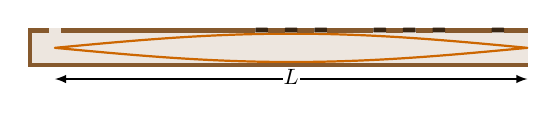
\begin{tikzpicture}
  \draw[<->] (0,-1.8*\R) --++ (\L,0)
    node[midway,below=-4,fill=white,inner sep=0.5,scale=0.8] {$L$};
  \wave{1}{1}
  \holes{1,3,4,5,7,8,9}
\end{tikzpicture}

% C5 - octave up
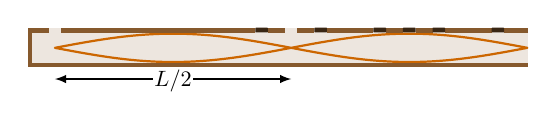
\begin{tikzpicture}
  \draw[<->] (0,-1.8*\R) --++ (\L/2,0)
    node[midway,below=-4,fill=white,inner sep=0.5,scale=0.8] {$L/2$};
  \wave{1}{2}
  \holes{1,3,4,5,7,9}
\end{tikzpicture}

% E - 4/5 - major third
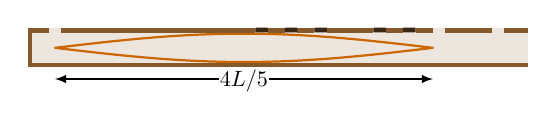
\begin{tikzpicture}
  \draw[<->] (0,-1.8*\R) --++ (4/5*\L,0)
    node[midway,below=-4,fill=white,inner sep=0.5,scale=0.8] {$4L/5$};
  \wave{4/5}{1}
  \holes{4,5,7,8,9}
\end{tikzpicture}

% F - 3/4 - perfect fourth
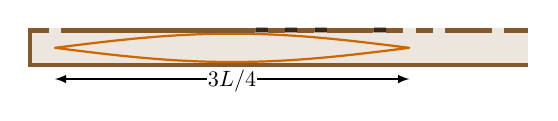
\begin{tikzpicture}
  \draw[<->] (0,-1.8*\R) --++ (3/4*\L,0)
    node[midway,below=-4,fill=white,inner sep=0.5,scale=0.8] {$3L/4$};
  \wave{3/4}{1}
  \holes{5,7,8,9}
\end{tikzpicture}

% F - 3/4 - perfect fourth
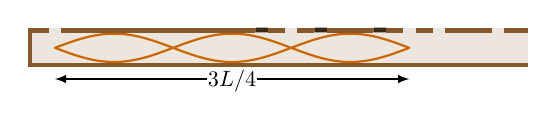
\begin{tikzpicture}
  \draw[<->] (0,-1.8*\R) --++ (3/4*\L,0)
    node[midway,below=-4,fill=white,inner sep=0.5,scale=0.8] {$3L/4$};
  \wave{3/4}{3}
  \holes{5,7,9}
\end{tikzpicture}

% C5 - octave up
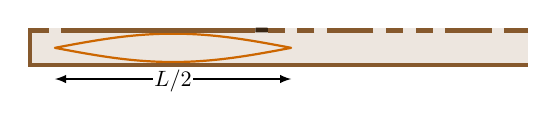
\begin{tikzpicture}
  \draw[<->] (0,-1.8*\R) --++ (\L/2,0)
    node[midway,below=-4,fill=white,inner sep=0.5,scale=0.8] {$L/2$};
  \wave{0.5}{1}
  \holes{9}
\end{tikzpicture}

\end{document}